\documentclass[english]{beamer}
\usetheme{default}
\usepackage{lmodern}
\usepackage[utf8]{inputenc}
\usepackage[T1]{fontenc}
\usepackage{babel}
\usepackage{color}
\usepackage{listings}
\usepackage{booktabs}
\usepackage{amsmath,amsthm,amssymb,graphicx,mathrsfs}
\usepackage{stmaryrd}
\usepackage{slashed}
%\usepackage[hmargin={3.5cm,3.5cm},top=4cm,bottom=4cm]{geometry} %problem...

\graphicspath{{images/}}

\newcommand{\vb}[1]{\mathbf{#1}}
\newcommand{\V}[1]{\textnormal{#1}}
\newcommand{\dd}[0]{\textrm{d}}
\newcommand{\bra}[1]{\langle#1 |}
\newcommand{\ket}[1]{| #1 \rangle}
\newcommand{\vdot}[0]{\boldsymbol\cdot}
\newcommand{\dom}{\mathrm{Dom}}

\newtheorem{remark}{Remark}
\newtheorem{proposition}{Proposition}

\setbeamertemplate{footline}[frame number]{}
\setbeamertemplate{navigation symbols}{}
\setbeamertemplate{caption}[numbered]


%%%%%%%%%%%%%%%%%%%%%%%%%%%%
\lstset{%
  backgroundcolor=\color{white},   % choose the background color; you must add \usepackage{color} or \usepackage{xcolor}
  basicstyle=\small,        % the size of the fonts that are used for the code
  commentstyle=\color{blue},    % comment style
  extendedchars=true,              % lets you use non-ASCII characters; for 8-bits encodings only, does not work with UTF-8
  keepspaces=true,                 % keeps spaces in text, useful for keeping indentation of code (possibly needs columns=flexible)
  keywordstyle=\color{red},       % keyword style
  language=Fortran,                 % the language of the code
  rulecolor=\color{black},         % if not set, the frame-color may be changed on line-breaks within not-black text (e.g. comments (green here))
  showspaces=false,                % show spaces everywhere adding particular underscores; it overrides 'showstringspaces'
  showstringspaces=false,          % underline spaces within strings only
  showtabs=false,                  % show tabs within strings adding particular underscores
  stringstyle=\color{green},     % string literal style
  tabsize=2,                       % sets default tabsize to 2 spaces
  frame=single
}



%%%%%%%%%%%%%%%%%%%%%%%%%%%%%%%%%%%%%%%%%%%%%%%%%%%%%%%%%%%%%%%%%%%%%%%%
\title{Boundary and matching conditions for quantized Dirac fields}
\author{En-Hung CHAO}
\institute{{\'E}cole Polytechnique \& Universit{\"a}t Leipzig}
\date{September 4th 2017}
%%%%%%%%%%%%%%%%%%%%%%%%%%%%%%%%%%%%%%%%%%%%%%%%%%%%%%%%%%%%%%%%%%%%%%%%
%%%%%%%%%%%%%%%%%%%%%%%%%%%%%%%%%%%%%%%%%%%%%%%%%%%%%%%%%%%%%%%%%%%%%%%%
\begin{document}
%\selectlanguage{english}
%\graphicspath{{../images/}}

\begin{frame}
\titlepage%
\centerline{supervised by Jochen Zahn (Universit{\"a}t Leipzig)}
\end{frame}
%%%%%%%%%%%%%%%%%%%%%%%%%%%%%%%%%%%%%%%
%%%%%%%%%%%%%%%%%%%%%%%%%%%%%%%%%
\begin{frame}
\frametitle{Outline}
\framesubtitle{}

\begin{enumerate}

\item Introduction
\item Vacuum polarization in the presence of a Kondo-type potential
\item Generalization of Wentzell boundary condition for massless fermions
\item Conclusion

\end{enumerate}

\end{frame}
%%%%%%%%%%%%%%%%%%%
\begin{frame}
\frametitle{Introduction}
\framesubtitle{}

\begin{itemize}
\item<1-> Well-posedness of Cauchy problem with the matching and boundary conditions
\item<2-> Vacuum polarization 
	\begin{itemize}
		\item Define the vacuum expectation of the current density as a Hadamard state
		\item Renormalization by point-splitting w.r.t the Hadamard parametrix
	\end{itemize}
\end{itemize}

\end{frame}
%%%%%%%%%%%%%%%%%%
\begin{frame}[shrink=30]
\frametitle{\small{Vacuum polarization in the presence of a Kondo-type delta potential}}
\framesubtitle{}
\begin{itemize}
%
\item<1-> 
The equation of motion for a massless spin-$\frac 1 2$ fermion in the presence of a Kondo-type potential in $\mathbb{R}\times[-\frac L 2 , \frac{L}{2}]$\\
\tiny\color{blue}[J. Erdmenger, C. Hoyos, A. O'Bannon and J. Wu, JHEP
, 12:086, 2013]\color{black}\normalsize

\begin{equation*}
i \partial_0 \phi = 
\underbrace{\begin{pmatrix} 
-1 & 0 \\
0 & 1 
\end{pmatrix} i \partial_1 \phi }_{H\phi}+
\begin{pmatrix}
v_3 & v_- \\
v_+ & -v_3
\end{pmatrix} \delta(x^1) \phi
\end{equation*}
where $\phi = \gamma^0\psi$ for some Dirac field $\psi$,  $v_3, v_+ + v_- \in \mathbb{R}$ and $ v_+ - v_-\in i \mathbb{R}$
%
\item<2-> Matching condition (m.c.) at $x^1 = 0$ 
%
\item<3-> Bag boundary condition (b.d.c.) for confined cases 
\begin{equation*}
- i\gamma^1 \phi \Big\vert_{\pm \frac{L}{2}} = \pm \phi \Big\vert_{\pm \frac{L}{2}}
\end{equation*}

%
\item<4-> In the confined case, the problem $i\partial_0\phi = H\phi$ is well posed since $H$ is an essentially self-adjoint operator of the Hilbert space
\begin{equation*}
\mathcal{H} = L^{2}\Big(\big[-\frac L 2, 0\big), \mathbb{C}^2\Big) \oplus L^{2}\Big(\big(0,\frac L 2\big], \mathbb{C}^2\Big) 
\quad,\quad
\langle \cdot, \cdot\rangle_{\mathcal{H} } = \langle \cdot, \cdot\rangle_{L^{2}\big(\big[-\frac L 2, 0\big), \mathbb{C}^2\big)} +\langle \cdot, \cdot\rangle_{L^{2}\big(\big(0,\frac L 2\big], \mathbb{C}^2\big)}
\end{equation*}

 on the domain
\begin{equation*}
\mathrm{Dom}(H) = \Big \{\phi \enskip \big\vert \enskip \phi \in C^{1}(I_-, \mathbb{C}^2) \oplus C^{1}(I_+, \mathbb{C}^2), \enskip \phi \textrm{ b.d.c + m.c.} \Big \}
\end{equation*} 


\end{itemize}
\end{frame}
%%%%%%%%%%%%%%%%%%
\begin{frame}[shrink=30]
\frametitle{\small{Vacuum polarization in the presence of a Kondo-type potential}}
\framesubtitle{Definition of vacuum current and stress-energy tensor}

\begin{itemize}
\item<1-> Define the Hadamard state
\\\tiny\color{blue}[J. Schlemmer and J. Zahn, Ann. of Phys. 2015]\color{black}\normalsize
\begin{equation*}
\begin{split}
\omega(\psi^B(x)\bar{\psi}_A(y)) = & \int_{E_k >0} \psi_k^B(x)\bar{\psi}_{A,k}(y)e^{-i(x^0-y^0)E_k} \dd k \\
\omega(\bar{\psi}_A(y)\psi^B(x)) = & \int_{E_k <0} \psi_k^B(x)\bar{\psi}_{A,k}(y)e^{-i(x^0-y^0)E_k} \dd k 
\end{split}
\end{equation*}
%
\item<2-> Renormalized vacuum current expectation
\begin{equation*}
j^\mu(x) = \lim_{y \rightarrow x} \gamma^A_B \big(
\omega(\psi^B(x)\bar{\psi}_A(y)) - H^B_A (x, y)\big)
\end{equation*}

%
\item<3-> Renormalized vacuum stress-energy tensor expectation

\begin{equation*}
\begin{split}
& T_{00} = \frac{i}{2} (\bar{\psi} \gamma_1 \nabla_1 \psi - \nabla_1 \bar{\psi}\gamma_1 \psi) , \quad
 T_{11} = \frac{i}{2} (\bar{\psi} \gamma_0 \nabla_0 \psi - \nabla_0 \bar{\psi}\gamma_0 \psi)  \\
& T_{01} = \frac{i}{4} (\bar{\psi} \gamma_1 \nabla_0 \psi +\bar{\psi} \gamma_0 \nabla_1 \psi - \nabla_1 \bar{\psi}\gamma_0 \psi - \nabla_0 \bar{\psi}\gamma_1 \psi)  
\end{split}
\end{equation*}

\begin{equation*}
\begin{split}
T_{00}(x,y) = 
\frac{i}{2}\Big( & 
\nabla_{x^1}\big(\omega(  \psi^B(x) \bar{\psi}_A(y))-H^B_A(x,y)\big)(\gamma_1)^A_B \\
& - \nabla_{y^1}\Big(\omega( \psi^B(x)  \bar{\psi}_A(y)) - H^B_A(x,y)\big)(\gamma_1)^A_B \Big)   
\end{split}
\end{equation*}

\end{itemize}
\end{frame}
%%%%%%%%%%%%%%%%%%%%%%%%%%%%%%%%%%%%%%

\begin{frame}[shrink=30]
\frametitle{\small{Vacuum polarization in the presence of a Kondo-type potential}}
\framesubtitle{}

\begin{itemize}

\item<1-> Confined and with constant external electric field $E$ with static gauge for the vector potential $A^\mu(x) = (Ex^0, 0)$

\begin{itemize}
\item<2-> Eigenvalues of $H_E = H + eEx^1 $ (modes)
\begin{equation*}
k_{n} = \frac{(-1)^n}{L}  \theta + \frac{2\pi}{L}n 
\end{equation*}
where $\theta = \theta(E, v_3, v_+, v_-)$
%
\item<3-> Vacuum polarization and stress-energy tensor
\begin{equation*}
\rho(x) = \frac{e}{\pi L}\Big( \frac{\beta \sin \theta \cos \eta}{\alpha + \beta \sin \eta \cos \theta}\Big) (-\theta + \pi)
\Big(\Theta(- x^1) - \Theta(x^1))\Big) + \frac{e^2 E}{\pi} x^1
\end{equation*}
%
\begin{equation*}
T_{\mu\nu}(x) = 
\bigg( \frac{\pi}{2L^2}\big( -\frac{1}{3} + \frac{(\theta - \pi)^2}{\pi^2}\big) + \frac{e^2E^2(x^1)^2}{2 \pi} \bigg)
\begin{pmatrix}
1 & 0 \\ 0 & 1
\end{pmatrix}
\end{equation*}
%
\item<3-> When $v_3 = v_\pm = E = 0$, we obtain the same result for the stress-energy tensor for Casimir effect \\
\tiny\color{blue}[P. Sundberg and R. L. Jaffe, Annals Phys., 309:442?458, 2004]\normalsize\color{black}
\end{itemize}
%
\item Non-confined case
\begin{itemize}
\item<4-> Wave functions are normalized to $\delta$-function.
\item<5-> Same results at $L\rightarrow +\infty $ limit.
\end{itemize}

\end{itemize}

\end{frame}
%%%%%%%%%%%%%%%%%%
\begin{frame}[shrink=30]
\frametitle{\small{Generalization of Wentzell boundary condition for massless fermions}}
\framesubtitle{}

$\mathcal{M}$ a d+1 dimensional spin manifold (Minkowski) with time-like static boundary $\partial\mathcal{M}$

\begin{itemize}
\item<2-> We consider the action

\begin{equation*}
\mathcal{S} = \frac{1}{2}i\int_{\mathcal{M}} \bar{\psi} \gamma^\mu \partial_\mu \psi - \partial_\mu \bar{\psi} \gamma^\mu \psi 
+ \frac{1}{2}\int_{\partial \mathcal{M}} ic \bar{\psi} \gamma^\alpha \partial_\alpha (1 - i \gamma^\bot) \psi
+ \bar{\psi} \psi
\end{equation*}
%motivated by holographic renormalization \\
where $\gamma^\bot = n_j\gamma^j$ with $n$ unit inward vector normal to the boundary.\\
\tiny\color{blue}[M. Henningson and K. Sfetsos,
Phys. Lett. B, 431(1):63-68, 1998
] \color{black}\normalsize
\tiny\color{blue} [R. Contino and A. Pomarol JHEP, 11:058, 2004]
\color{black}\normalsize
%
%
\item<3-> EOM in terms of $\phi = \gamma^0 \psi$
\begin{equation*}
\begin{cases}
i \partial_0 \phi = i \gamma^0 \gamma^j \partial_j \phi   \quad \textrm{in $\mathcal{M}$}\\
i \partial_0(1 + i\gamma^\bot) \phi = i\gamma^0 \gamma^a \partial_a (1+ i\gamma^\bot)\phi - c^{-1} \gamma^0(1 - i \gamma^{\bot})\phi \quad \textrm{on $\partial \mathcal{M}$}
\end{cases}
\end{equation*}
%
\item<4-> Bag boundary condition when $c\rightarrow0$ 
%
\item<5-> On the Hilbert space 
\begin{equation*}
\mathcal{H} = L^{2}(M,E)\oplus L^{2}(\partial M, \mathcal{P}_+ E) \quad,\quad
\langle \cdot, \cdot \rangle _\mathcal{H} = \langle \cdot, \cdot \rangle _{L^2(M)} + c \langle \cdot, \cdot \rangle _{L^2(\partial M)}
\end{equation*}
 where $M$ is an equal-time hypersurface of $\mathcal{M}$ and $\partial M = M\cap \partial \mathcal{M}$, we define


\begin{equation*}
\Delta = \begin{pmatrix}
i \gamma^0 \slashed{\partial}  & 0 \\
-c^{-1} \gamma^0 \mathcal{P}_- \cdot \vert_{\partial M}&  i\gamma^0 \slashed{\partial}_| \mathcal{P}_+
\end{pmatrix}
\end{equation*}
where $\slashed{\partial} = \gamma^j\partial_j$ for
$j \in \llbracket 1 , d \rrbracket$, $\slashed{\partial}_| = h^{ab} \gamma_{a} \partial_{a}$ where $h$ is the induced metric on the boundary and $
\mathcal{P}_\pm = \frac{1}{2}(1 \pm i n_j\gamma^j) $
is a Hermitian projector.

\end{itemize}

\end{frame}
%%%%%%%%%%%%%%%%%%
\begin{frame}[shrink=40]
\frametitle{\small{Generalization of Wentzell boundary condition for massless fermions}}
\framesubtitle{}

\begin{itemize}

\item<1-> $\Delta$ is self-adjoint on the domain

\begin{equation*}
\dom( \Delta) = \{ \Phi = (\phi, \phi_|) \in W^{1,2}(M)\times W^{1,2}(
\partial M) \enskip | \enskip \mathcal{P}_+\phi \vert_{\partial M} - \phi_| = 0 \} 
\end{equation*}  

$\Rightarrow$ unitary time evolution.
\newline

\item<2-> \textbf{Causal propagation}\\
%We denote
%\begin{equation*}
%\mathcal{H}^k(M) = \cap_{s=0}^{k} \dom(\Delta), 
%\quad
%\| \cdot \|_{\mathcal{H}^k(M)} = \| \Delta^k \cdot \|_{\mathcal{H}(M)}
%\end{equation*}

\begin{proposition}\label{wen-prop-causal}
Suppose that 0 is an isolated point of the spectrum of $\Delta$. 
Let $\Sigma_0$ and $\Sigma_1$ be two equal-time surfaces.
Let $\Phi_0 = (\phi_0, \phi_{|0})\in W^{\infty,2}(M)\times W^{\infty,2}(\partial M)$ be the initial data of the problem such that
\begin{equation}\label{wen-domaindeltak}
\begin{split}
& \mathcal{P}_-\big( \partial_\bot^{2k-1}\phi\vert_{\partial M} - c^{-1}\partial_\bot^{2k-2}\phi\vert_{\partial M}\big) = 0  \\
& \mathcal{P}_+\big( \partial_\bot^{2k}\phi\vert_{\partial M} - c^{-1}\partial_\bot^{2k-1}\phi\vert_{\partial M}\big) =0  
\end{split}
\end{equation}
for all $k\in\mathbb{N}$.
Then, the solution $\Phi$ of the problem depends smoothly and causally on the initial data $\Phi_0$ in the sense that for any $\mathcal{S}_0 \subset \Sigma_0$
\begin{equation}
\big\| \frac{\partial^k}{\partial t^k} \Phi\big\|_{\mathcal{H}(\mathcal{S}_1)}
\leq
\big\| \Phi\big\|_{\mathcal{H}^{k}(\mathcal{S}_0)}
\end{equation}
for any $k\in\mathbb{N}$ and $\mathcal{S}_1 \in D^+(\mathcal{S}_0)\cap\Sigma_1$, where $D^+(\mathcal{S}_0)$ is the future domain of dependence of $\mathcal{S}_0$.
Here, the rhs of the inequality represents the norm of the restriction of $\frac{\partial^k}{\partial t^k} \Phi$ on $\mathcal{S}_1$ and the lhs is defined by $\|\Delta^k \Phi\|_{\mathcal{H}(\mathcal{S}_0)}$  
\end{proposition}

\item<3-> Two examples 

	\begin{itemize}
		\item<4-> $M = \mathbb{R}^{d-1}\times \mathbb{R}_+$ the spectrum is $\mathbb{R}$
		\item<5-> $M = \mathbb{R}^{d-1}\times [-L, L]$ the spectrum is
		\begin{equation*}
		\{k\in\mathbb{R} \enskip\vert\enskip k^2 = p^2 + q^2 \enskip\mathrm{ where }\enskip p\in\mathbb{R}^{d-1}, \tan q L = \frac{\mp q + c^{-1}}{q \pm c^{-1}}\}
		\end{equation*}
		$\Rightarrow$ Causal propagation in $d=1$
	\end{itemize}
\end{itemize}

\end{frame}
%%%%%%%%%%%%%%%%%%
\begin{frame}[shrink=30]
\frametitle{\small{Generalization of Wentzell boundary condition for massless fermions}}
\framesubtitle{}

\begin{itemize}

\item<1-> Shock-wave solution in $\mathcal{M} = \mathbb{R}^{1,1}\times\mathbb{R}_+$ $\Phi = (\phi, \phi_|)$
where
\begin{equation*}
\phi = \begin{pmatrix}
i \big(\delta(x^0 - x^2) + \delta(x^0 + x^2) - 4c^{-1}\Theta(x^0-x^2)e^{- \frac{x^0-x^2}{c}} \big) \\
\delta({x^0 - x^2}) - \delta(x^0 + x^2) - 4c^{-1}\Theta(x^0-x^2)e^{- \frac{x^0-x^2}{c}} \end{pmatrix}
\end{equation*}
\begin{equation*}
\phi_| = \mathcal{P}_+ \phi\vert_{\partial \mathcal{M}} = 
\begin{pmatrix} 0 \\ -4c^{-1}e^{- \frac{x^0}{c}} \Theta(x^0) \end{pmatrix}
\end{equation*}


\item<2-> Vacuum energy density in $\mathcal{M} = \mathbb{R}\times [-L, L] $ under our boundary condition
	%\begin{itemize}
	%\item<3-> The spectrum is discrete and symmetric wrt 0
	%\begin{equation*}
	%2kL + 2\arctan ck = \big(n + \frac 1 2 \big)\pi \quad\mathrm{for } n\in\mathbb{Z}
	%\end{equation*}
	%\item<4->
	%$\rho = 0$
	%\item<3-> Relation between energy density $T_{00}$ and the coupling constant 
		
	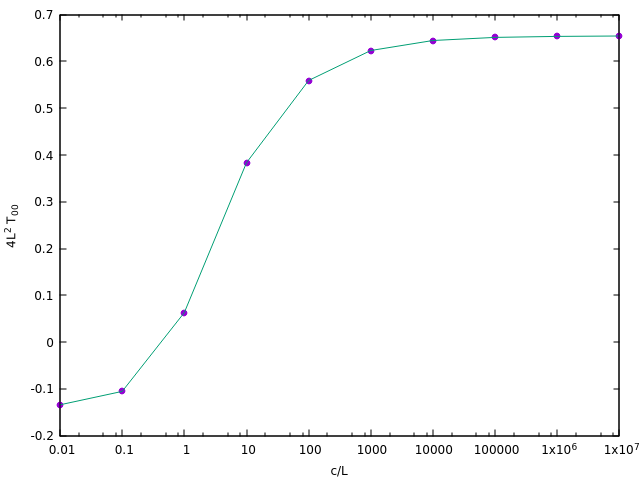
\includegraphics[scale=0.5]{T00}\centering

	%\end{itemize}


\end{itemize}

\end{frame}
%%%%%%%%%%%%%%%%%%

\begin{frame}[shrink=0]
\frametitle{Conclusion and perspectives}
\framesubtitle{}

\begin{itemize}
\item<1-> To summarize
	\begin{itemize}
	\item<2-> A Kondo-type potential creates a discontiunuous background vacuum charge density and shifts the vacuum energy density by a constant.
	\item<3-> Wentzell boundary condition can be generalized to the case of massless fermions.
	\item<4-> The causal propagation property of free massless fermions with Wentzell boundary condition holds on certain manifolds.
	\item<5-> The influence of the coupling constant of Wentzell boundary condition over the energy density has been shown for 1+1 dimension.
	\end{itemize}
\item<6-> Outlooks
	\begin{itemize}
	\item Generalization of Wentzell boundary condition to vector fields and gauge fields
	\item Generalization to the massive case where the causal propagation property is supposed to be more widely valid.
	\end{itemize}
\end{itemize}
\end{frame}
\end{document}

















